\section{Materials and methods}
\label{sec:methods}

\subsection{Design overview}

CascadeBench measures how acoustic channel degradations propagate through
commercial speech recognition and translation services that can only be
accessed through their public interfaces. The design is shown in
Fig.~\ref{fig:arch}. A bilingual corpus of 480 sentences is synthesised to
audio with multiple neural voices, degraded by a grid of controlled channel
impairments, and submitted to five recognition systems and four speech
translation paths. Every stage of the pipeline is scripted with fixed random
seeds, and every model response together with its round-trip latency is
logged at the sentence level, so that the complete measurement can be
re-executed as providers update their services.

\begin{figure}[t]
\centering
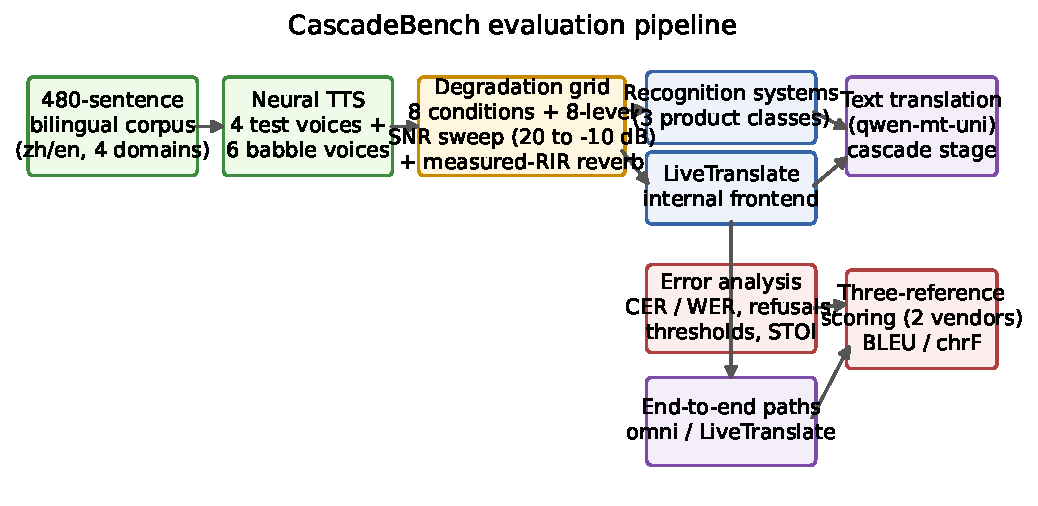
\includegraphics[width=\textwidth]{../figures/fig1_architecture.pdf}
\caption{Architecture of the CascadeBench evaluation pipeline. A stratified
bilingual corpus is synthesised with multiple neural voices, degraded by a
grid of eight acoustic channel conditions plus a noise severity sweep, and
processed by recognition systems from three architectural families. Cascade
systems forward recogniser output to a text translation engine; end-to-end
systems translate audio directly.}
\label{fig:arch}
\end{figure}

\subsection{Corpus}

The corpus contains 240 Mandarin Chinese and 240 English sentences, balanced
across four content domains and three length strata, twenty sentences per
cell. The domains are broadcast news, everyday conversation, technical and
scientific exposition, and a numerals-and-entities stratum rich in dates,
quantities, addresses, and named entities, which is known to stress
recognition and inverse text normalisation. Short sentences contain 8 to 14
Chinese characters or 5 to 9 English words, medium sentences 15 to 25
characters or 10 to 17 words, and long sentences 26 to 39 characters or 18 to
24 words. The mean length is 19.3 characters for Chinese and 12.0 words for
English. Sentences were authored to be self-contained and
factually neutral, to avoid brand names and transliterated loanwords whose
recognition would depend on provider-specific vocabulary rather than on
acoustic processing, and to distribute numerical expressions across date,
time, quantity, price, and identifier formats within the numerals domain. All numbers are written out in words in the corpus text, for example
two thousand twenty five, so that the spoken realisation is unambiguous and
the reference transcript matches the synthesis input exactly.

Each sentence was synthesised by a neural speech synthesis service (Sambert,
Alibaba Cloud Model Studio) using two distinct voices per language, a male
and a female voice for Chinese and two native-sounding voices for English,
with sentences alternating between the voices so that each voice realises 120
sentences per language. Synthesis produced 16~kHz single-channel PCM audio.
The 44 babble noise source tracks described below were synthesised with six
additional voices that are disjoint from the four test voices. Using
synthesis rather than recorded speech has two methodological advantages. The
reference transcript is exact by construction, which removes the transcription
noise that limits error floor measurement in recorded corpora, and the
acoustic properties of the test material can be regenerated at any time,
which decouples the benchmark from the licensing and availability constraints
of recorded corpora such as AISHELL-1~\cite{bu2017aishell} or
LibriSpeech-derived material~\cite{zen2019libritts}. The corresponding
limitation, that synthetic speech does not sample the full variability of
spontaneous human speech, is examined in Section~\ref{sec:limitations}.

\subsection{Acoustic degradation grid}

Eight channel conditions plus the clean control form the main grid. The
conditions were selected to span the canonical impairment families that
speech services encounter between a talker and a data centre.

Additive babble noise is the most extensively sampled family. Babble was
constructed by concatenating randomly selected segments from the 44 disjoint
noise-source tracks described above, mixing three such streams, and
normalising the mixture, which produces speech-shaped noise with realistic
spectral and temporal structure rather than stationary synthetic noise. Speech-shaped interference was chosen over stationary
noise because it is the harder and the more ecologically valid case: babble
exhibits the temporal modulation and spectral occupancy of competing talkers,
masking the target in the same time-frequency regions that carry linguistic
information, whereas stationary noise is partly countered by any
spectral-subtraction-style front-end that a provider may have deployed
internally. The
noise was scaled against the active-speech level of each utterance, measured
as the mean energy of frames above the 60th energy percentile, to hit target
signal-to-noise ratios of 20, 15, 10, 5, and 0~dB. Calibration was verified
by re-measuring the realised signal-to-noise ratio of the mixed signals
against the clean signal; the realised values matched the targets within
0.1~dB on average. The 10~dB and 0~dB points enter the main grid, and the
full five-point ladder forms the severity sweep on a stratified 144-sentence
subset, 72 sentences per language, sampled evenly from every
domain-by-length cell.

Reverberation was applied by convolving each signal with a synthetic room
impulse response of the exponentially decaying noise
form~\cite{allen1979image,habets2006room} with a direct-path impulse and a
reverberation time of 0.5~s, which corresponds to an ordinary reverberant
room rather than an extreme auditorium. Narrowband degradation resamples each
signal to 8~kHz and back to 16~kHz, which removes the 4 to 8~kHz band exactly
as a telephone channel does; the telephone-specialised recogniser receives
the 8~kHz signal natively. Codec degradation encodes each signal with the
Opus codec~\cite{valin2012definition} at 8~kbit/s mono and decodes it back,
emulating an aggressive but deployed voice-over-IP setting. Packet loss
zeroes 15 percent of 20~ms frames chosen uniformly at random, emulating
lossy transport without jitter compensation. Clipping applies hard amplitude
limiting at 0.3 of full scale. Tempo distortion resamples the time axis by a
factor of 1.15 with pitch preservation, emulating playback-speed variation
or time-scale modification upstream of the service. All random draws use
per-sentence and per-condition seeds derived deterministically from the
sentence identifier and condition name, so the degraded signals are bitwise
reproducible.

Formally, for a clean signal $x[n]$ of length $N$ and a babble realisation
$b[n]$, the mixed signal at level $\rho$~dB is
\begin{equation}
y[n] = x[n] + \sigma\, b[n], \qquad
\sigma = \sqrt{\frac{P_{\mathrm{act}}(x)}{10^{\rho/10}\, \overline{P}(b)}},
\label{eq:snr}
\end{equation}
where $\overline{P}(b)$ is the mean power of the babble and
$P_{\mathrm{act}}(x)$ is the active-speech power estimated from frames whose
energy exceeds the 60th energy percentile of the utterance, which
approximates the ITU-T P.56 active-level convention with a fixed percentile
rule. The reverberation impulse response is
\begin{equation}
h[n] = \delta[n] + v[n]\, e^{-6.9\, n / (f_s T_{60})}, \qquad n = 0, \dots,
\lceil f_s T_{60} \rceil,
\label{eq:rir}
\end{equation}
with $v[n]$ unit-variance white noise, $f_s = 16$~kHz, $T_{60} = 0.5$~s, and
$h$ normalised to unit energy, and the reverberant signal is the truncated
convolution of $x$ with $h$ rescaled to the peak amplitude of $x$. Packet
loss zeroes each independent 20~ms frame with probability $p = 0.15$,
\begin{equation}
y[n] = m_k\, x[n], \quad n \in \text{frame } k, \qquad m_k \sim
\mathrm{Bernoulli}(1 - p),
\label{eq:pl}
\end{equation}
and clipping applies $y[n] = \operatorname{sign}(x[n]) \min(|x[n]|, 0.3)$.
Narrowbanding resamples by factors of one half and two with polyphase
anti-aliasing filters, codec degradation round-trips the signal through the
Opus encoder at 8~kbit/s, and tempo distortion applies a pitch-preserving
time-scale modification of factor 1.15.

\subsection{Systems under test}

Table~\ref{tab:systems} lists the systems. The recognition systems span
three architectural families as served by a single commercial provider
(Alibaba Cloud Model Studio, Beijing region) during October 2026, accessed
through their documented interfaces. The specialised family consists of
streaming recognisers in the Paraformer lineage~\cite{gao2023funasr}, a
16~kHz model and an 8~kHz telephone-band model. The LLM-ASR family consists
of Qwen-Audio 3.1 Flash~\cite{chu2024qwen2audio} and Qwen3-ASR Flash, audio
input models built on large language model backbones. The multimodal family
consists of Qwen3.8-Omni Flash, a general-purpose omni-modal foundation
model~\cite{qwen2.5omni2025} queried with a transcription instruction. All
systems were accessed in their default configurations, since a consumer of a
black-box service cannot apply front-end training or adaptation, and the
question of interest is precisely how the services behave out of the box.
The streaming recognisers were driven by streaming local audio over their
realtime WebSocket interface, sending each utterance as 16~kHz or 8~kHz PCM
frames at the maximum accepted rate and collecting sentence-final segments.
The LLM-ASR and omni systems received base64-encoded whole utterances in
their audio-input message format, the omni model together with an
instruction prompt for transcription or translation. The streaming
translation service was driven over its realtime interface with a session
configuration specifying text-only output and the target language, sending
raw PCM frames and collecting both the source transcript and the translated
text that the service emits, and the text translation engine received
source text with explicit source and target language tags. Every call was
executed with an automatic retry policy of up to six attempts with
exponential backoff on throttling, timeout, and connection failures, and no
other tuning parameters were exposed or set. The speech translation systems are the text translation
engine qwen-mt-uni, used as the second stage of two cascades built on the
16~kHz specialised recogniser and on the Qwen-Audio 3.1 recogniser, and two
end-to-end paths: the omni foundation model with an audio translation
instruction, and a dedicated streaming speech translation service
(LiveTranslate) that internally combines a streaming frontend recogniser
with a translation model. The internal frontend of the streaming translation
service, which its responses expose as source transcripts, is additionally
scored as a sixth recognition system. All API calls were executed on
free-tier quotas with the stop-on-exhaustion option enabled, which both
bounds the study at zero monetary cost and documents the practical quota
requirements of such a measurement.

\begin{table}[t]
\centering
\caption{Systems under test and their roles in the benchmark.}
\label{tab:systems}
\small
\begin{tabular}{llll}
\toprule
System (family) & Interface & Role & Evaluated on \\
\midrule
Paraformer-RT-v2 (specialised) & streaming ASR & recogniser & full grid \\
Paraformer-RT-8K-v2 (specialised, 8 kHz) & streaming ASR & recogniser & Chinese subset \\
Qwen-Audio-3.1-Flash (LLM-ASR) & audio input API & recogniser & full grid \\
Qwen3-ASR-Flash (LLM-ASR) & audio input API & recogniser & full grid \\
Qwen3.8-Omni-Flash (omni) & audio input API & recogniser, E2E ST & main grid \\
LiveTranslate frontend (specialised) & streaming ST & recogniser (internal) & sweep subset \\
qwen-mt-uni (MT) & text translation & cascade stage, oracle & full corpus \\
Qwen3.8-Max (LLM) & text generation & independent reference & full corpus \\
\bottomrule
\end{tabular}
\end{table}

\subsection{Evaluation protocol}

Recognition accuracy is scored as the character error rate (CER) for Chinese
and the word error rate (WER) for English, computed with the standard
Levenshtein alignment~\cite{levenshtein1966binary} after a normalisation
pipeline that is applied identically to references and hypotheses. The
normalisation performs Unicode compatibility folding, case folding,
punctuation removal, and, critically, canonicalisation of numeric
expressions. Because commercial recognisers differ in their inverse text
normalisation conventions, with the same spoken quantity rendered as twenty
six, 26, or two six depending on the system, both sides of every comparison
are mapped to a canonical digit form by rules that handle Chinese and
English cardinal numbers, digit-by-digit readings, time expressions, decimal
fractions, and scale multipliers such as wan and yi on the Chinese side and
million and billion on the English side, with ordinal expressions masked to
a common token. The rule set was developed and verified on the clean
condition, where residual normalisation artefacts were inspected sentence by
sentence until the clean-condition error rates reported in
Section~\ref{sec:results} reflect genuine recognition behaviour rather than
scoring artefacts. Utterances for which a service returns no transcript at
all, a behaviour documented in Section~\ref{sec:results}, are scored as
complete failures with an error rate of one.

Translation quality is scored with corpus-level BLEU~\cite{papineni2002bleu}
using sacreBLEU~\cite{post2018call} with the 13a tokeniser for English
targets and the character-level tokeniser for Chinese targets, and with
chrF~\cite{popovic2015chrf} as a second string-matching metric. Because the
corpus is direction-symmetric, BLEU is computed separately for the
Chinese-to-English and English-to-Chinese halves and macro-averaged. Every
hypothesis is scored against two reference sets. The primary reference is
produced by Qwen3.8-Max~\cite{qwen3technical2025}, a general-purpose LLM from
a different product family than any translation system under test, translating
the clean reference transcripts. The secondary reference is the oracle
cascade output, that is, the cascade translation engine applied to the clean
reference transcripts. The dual-reference design exposes a bias that
Section~\ref{sec:results:dual} quantifies: automatic scoring against
machine-generated references systematically favours systems from the same
model family as the reference generator, and conclusions about absolute
quality depend on the choice of reference, whereas conclusions about
degradation are stable.

Latency is measured as the wall-clock round trip of each API call from
dispatch to the complete response, recorded per call. For cascades, the
reported end-to-end latency is the sum of the recognition and translation
call latencies, which is the quantity a service consumer experiences when
the two stages are invoked sequentially. Streaming systems are fed audio at
the maximum rate their interface accepts, so the measurement reflects
service-side processing rather than client-side throttling.

\subsection{Experimental scale and cost}

The complete measurement comprises 26,238 successful API calls: 520
synthesis calls producing 31 minutes of source audio, 4,752 degraded
variants per recognition system covering 4.9 hours of audio, and 7,411
translation calls across the oracle, reference, cascade, and end-to-end
phases. Another 3,400 calls were consumed by retry attempts and by
connection resets of the realtime translation interface, which are counted
here because they represent real operational behaviour of the service. The
entire campaign ran on complimentary service quotas with the
stop-on-exhaustion option enabled, and one system, the omni translation
path, reached its free-tier limit before completing the severity sweep,
which bounds the end-to-end comparison to the main grid with 84 of the 144
sweep sentences per condition. The total wall-clock duration of data
collection was approximately four hours with up to five systems queried in
parallel. These figures are reported so that other laboratories can
estimate the feasibility of replicating or extending the measurement; they
also demonstrate that a full multi-system, multi-condition robustness
characterisation of commercial speech services is attainable at zero
monetary cost with careful quota budgeting, which lowers the barrier for
the periodic re-measurement that the field currently lacks.

\subsection{Statistical analysis}

All aggregate error rates and quality scores are reported with 95 percent
bootstrap confidence intervals over sentences, using 1000 resamples.
Differences between systems within a condition are tested with the Wilcoxon
signed-rank test~\cite{wilcoxon1945individual} on paired per-sentence errors,
with Holm correction~\cite{holm1979simple} across the family of pairwise
comparisons. Noise severity is modelled by ordinary least squares regression
of the error rate on the signal-to-noise ratio, with bootstrap confidence
intervals for the slope, and the slope is reported in percentage points per
dB as the degradation gradient of a system. The relationship between
recognition error and translation quality across operating conditions is
summarised by the cascade amplification coefficient, defined as the slope of
regressing the BLEU loss from the oracle against the mean recognition error
rate, together with its Pearson correlation; a slope near one with high
correlation indicates linear error pass-through, and the slope value itself
is the pass-through rate. Signal processing and statistics use
SciPy~\cite{virtanen2020scipy} and librosa~\cite{mcfee2015librosa}.
